\chapter{Application of Neural Networks for Object Detection}
In recent years, there has been an upsurge in the use of neural networks. We can partially attribute it to the evolution of hardware allowing for implementation of network models with multiple layers. Deep neural networks (DNNs) are now finding their use in many applications, e.g., classification, time series prediction, and optimization tasks, and are replacing many older machine learning methods. Some of the benefits of neural networks include their ability to find and learn complex non-linear relationships in provided data and subsequent generalization to unseen data. However, some applications do not allow for so-called \textit{black box} models and require a logical reasoning behind the decisions.

Image processing is one of the fields where DNNs are heavily utilized and outperform traditional machine learning approaches with big margins. Uses of DNNs for image processing vary from classification and object detection to auto-encoders for noise removal, and generative networks. A surge in DNN based image processing started in the 2010s with an implementation of a multi-layer convolutional network trained on GPU \cite{bib:deepOnGpu}. 

In this chapter, we take a closer look at how are DNNs applied in object detection. The goal of such a detector is to localize and classify multiple objects of interest in the given image. There are multiple ways of localization, such as semantic segmentation, which categorizes individual pixels, or key-point and skeleton detections. However, we are interested in more straightforward, axis-aligned bounding box (bbox) predictions. Each of the predicted bounding boxes needs a corresponding class prediction.

Considering the importance of classification in object detection, we dedicate a significant portion of this chapter to describing multiple classification network models. Many detection models directly utilize or are inspired by those classification networks. We also define metrics used to compare the performance of DNN models used for image processing.

\section{Metrics}
In order to evaluate and compare multiple approaches, we require clearly defined metrics. A state-of-the-art model presented without full specification of used evaluation metrics makes comparing multiple results impossible. Thankfully, there are competitions and challenges with precisely defined rules that are often used to make such comparisons. 

The \textit{ImageNet Large Scale Visual Recognition Challenge (ILSVRC)}\footnote{\url{http://www.image-net.org/challenges/LSVRC/}} is most often used to benchmark classification. Object detection is commonly evaluated in two challenges: the \textit{PASCAL Visual Object Classes Challenge}\footnote{\url{http://host.robots.ox.ac.uk/pascal/VOC/}}, and the \textit{COCO Object Detection Task}\footnote{\url{cocodataset.org/}}. Each challenge also provides a public dataset, \textit{ImageNet}, \textit{PASCAL VOC}, and \textit{COCO} respectively.

In this section, we define metrics used to evaluate those challenges, but also other, not considered qualities. Most notably, none of the mentioned challenges is evaluated based on the speed of the model. Because our work is focused on real-time video analysis, we are interested in finding a balance between accuracy and the number of images processed per second (fps). One more factor to consider would be the physical size of the model, usually represented by the number of parameters and directly impacting the amount of needed memory.

\subsection{Classification}
The most common and intuitive evaluation metric for classification problems is the number of correctly classified samples as a ratio of all samples. This ratio is referred to as a \textit{classification accuracy}. However, a complement to the accuracy, \textit{top-1 error}, is also often used. In \textit{ILSVRC},  alongside top-1 error, a \textit{top-5 error} is used as another major criterion. The top-5 error represents the fraction of test samples in which the correct label does not appear in the top 5 predicted results.

\subsection{Object detection}
Evaluating a localization and classification of multiple objects in image is a much complex task than simple classification, mainly because there is no simple one-to-one mapping between ground-truths and predictions. A ground-truth data are a set of \textit{N} boxes with labels, and detector generates a set of \textit{M} boxes with labels and class confidence values.

Because predicted boxes do not perfectly match ground-truths, a matching algorithm is needed to decide whether a prediction is true positive or false positive. Matching is usually done by computing intersection over union (IoU) value for each pair of ground-truth and predicted boxes, and then selecting positive detections based on predetermined threshold.
$$\text{IoU} = \frac{\text{Area}(\text{Prediction} \cap \text{Ground truth})}{\text{Area}(\text{Prediction} \cup \text{Ground truth})}$$

With predictions sorted into true positives (TP), false positives (FP) and false negatives (FN) (no predictions matching a ground-truth box) we are able to calculate \textit{precision} and \textit{recall}.
$$\text{Precision} = \frac{\text{TP}}{\text{TP}+\text{FP}} = \frac{\text{TP}}{\text{All predictions}}$$
$$\text{Recall} = \frac{\text{TP}}{\text{TP}+\text{FN}} = \frac{\text{TP}}{\text{All ground truths}}$$

Now we can define the first metrics used for object detection. Note that all following metrics depend on precision and recall, and therefore depend on the IoU threshold.

\subsubsection{Precision-Recall (PR) curve}
PR curve is simply a plot showing the relationship between values of precision and recall. It is plotted separately for each class, and reveals how much does a change in confidence, influence the precision and recall values. 

To create the curve, predictions for the given class are sorted by a confidence score. Then, for each prediction, precision and recall are calculated utilizing predictions with a higher confidence score. 

An object detector of a particular class is considered reliable if its precision stays high while recall increases. Meaning that predictions with lower confidence score can be considered good predictions.

\subsubsection{Average Precision (AP)}
Comparing curves is not an easy task, particularly if they cross each other frequently, as it often happens with PR curves. However, we can use the area under the PR curve as numerical metrics, called \textit{average precision}. It is calculated by interpolation, either on all data points or a small number of equally spaced points (\textit{PASCAL VOC Challenge} uses 11).

Interpolation equation for all points:
$$\sum_{r=0}^1 (r_{n+1} - r_n ) p_{interp}(r_{n+1})$$
with
$$p_{interp}(r) = \max_{\Tilde{r} \geq r} p(\Tilde{r})$$
where $p(\Tilde{r})$ is precision at recall $\Tilde{r}$.

\subsubsection{Mean Average Precision (mAP)}
Comparing two models class by class is impractical, especially with the classifiers for hundreds of classes. Therefore, the most often used metrics for object detectors is a \textit{mean average precision}. As the name suggests, it is a mean of AP across all classes. Most common notation, mAP@[0.5] means mAP with IoU threshold 0.5. The mAP can also be averaged over multiple IoU thresholds, mAP@[.5, .95] denotes the average mAP from IoU 0.5 to 0.95 usually with step 0.05.

\subsection{Inference time}
Inference time is a significant factor to consider for the model in real-time application use. With the state-of-the-art models, images are often processed under a second, often in a few milliseconds. Such small numbers can be hard to comprehend. Therefore a more intuitive metrics is used. That being the number of processed \textit{frames per second} (fps). However, unlike precision metrics, the fps values are heavily dependant on hardware, software framework, batch size and amount of pre- and post-processing included in the measurement. Hence, only the measurements performed in the identical hardware and software environment are suitable for comparison.

\section{Classification networks}
\label{sec:clsnets}
A fundamental building block for a modern state-of-the-art image classification network is a convolutional layer. Accordingly, we call this type of networks a convolutional neural networks (CNNs) \cite[ch.~9]{bib:dlbook}. CNN based classifier is a network that given the input image, extracts a feature map from this image and then applies classification layers to produce a confidence score for each possible class. Usually, the soft-max function is applied to the confidence score to get a probability distribution.

We use this section to take a walk through the history of classification CNNs and outline some of the most important models. Some of those models are still used, and others are responsible for inspiring the next generations of even better networks.

\subsection{AlexNet (2012)}
\textit{AlexNet} designed by \citeauthor{bib:alexnet} \cite{bib:alexnet} is the first CNN that won the \textit{ILSVRC} challenge over traditional computer vision and machine learning approaches. It created a foundation on which today's state-of-the-art models are built, and set a new standard for image recognition. \textit{AlexNet}'s model is a stack of five convolutional layers interleaved by max-pooling layers, followed by two fully connected layers and a softmax layer. It also popularized the use of ReLU non-linearity in CNNs.

\subsection{VGG (2014)}
\label{sec:VGG}
The network architecture, mostly known as \textit{VGG}, by \citeauthor{bib:vgg} \cite{bib:vgg}, is build onto the deep CNN concept behind \textit{AlexNet}. It managed to prove the feasibility of even deeper network utilizing small convolution filters. 

Each of the \textit{VGG's} convolutional filters employs a 3$\times$3 kernel with the depth of the feature map gradually increasing through the network. The convolutions are followed by three fully connected layers and softmax layer, see \cref{tab:vggarch}. 

Multiple versions of the \textit{VGG} architecture can be constructed, depending on the number of convolutional layers. The most popular is the 16 layer version, dubbed \textit{VGG-16}.

Today the \textit{VGG} network is considered to be a general architecture for a classification network due to its linear architecture with a decreasing area of the features, and an increasing number of channels. 

\begin{table}
    \centering
    \rotatebox{90}{
        \vggArch
    }
    \caption{Architecture of VGG network version D, commonly called VGG-16. Taken from \cite[table 1]{bib:vgg}}
    \label{tab:vggarch}
\end{table}
    
\subsection{Inception (2014)}
\label{sec:inception}
Predating architectures suggest that increasing the number of layers and layer size, leads to better precision. \citeauthor{bib:googlenet} introduced \textit{Inception v1} \cite{bib:googlenet}, also known as \textit{GoogLeNet}, with the goal of increasing precision while improving utilization of computing resources.

Although stacking more convolutional layers increases the accuracy, a growing computational cost of those layers quickly overpowers the benefits. To avoid the aforementioned cost, \textit{Inception} introduces the concept of sparsity in convolutional layers. It achieves sparsity by using \textit{inception modules} that approximate a sparse structure by using multiple convolutions with different kernel sizes and concatenating the outputs together, \cref{fig:incept_mod}. To further reduce the computational cost, each convolution is preceded with additional 1$\times$1 convolution, used for a dimensionality reduction. An alternate path in the inception module is provided by max-pooling operation and concatenating it to the output.

\textit{Inception} begins with a sequence of convolution, pooling, and local response normalization operations. This 'stem' is followed by a chain of nine inception modules, topped by a fully connected soft-max classifier. Two auxiliary classifiers are added to intermediate layers of the network to help propagate gradients and provide regularization during the training.

A set of improvements to the \textit{Inception} network is introduced in later versions of the network. Most notably a factorization of convolution layers in Inception v2 and v3, \citeauthor{bib:inception2} \cite{bib:inception2}. Factorization replaces larger convolutions with a network of multiple smaller ones. They found this method very effective, e.g., replacing a 5$\times$5 convolution with two layers of 3$\times$3 results in a relative gain of 28\% and replacing 3$\times$3 layer with 3$\times$1 and subsequent 1$\times$3 layer is 33\% cheaper.

\begin{figure}
    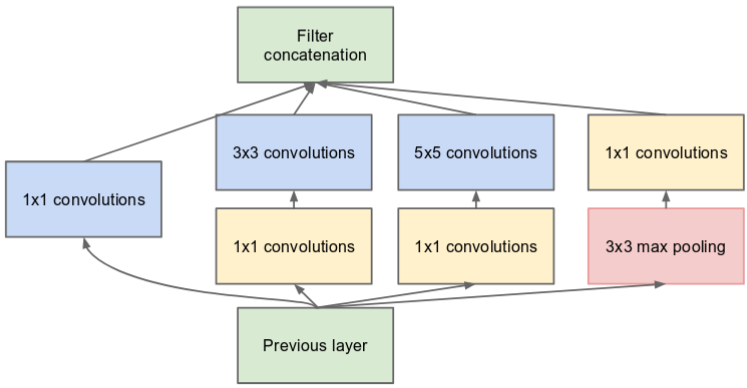
\includegraphics[width=\textwidth]{img/inception}
    \caption{Inception module, picture from \cite[figure 2]{bib:googlenet}.}
    \label{fig:incept_mod}
\end{figure}

\subsection{ResNet (2015)}
\label{sec:resnet}
A trend of adding more layers to CNNs to achieve better accuracy has pushed the limit towards networks with hundred or more layers.  Theoretically, adding more layers to a model should produce equal or better results, based on the fact that shallow model is the subspace of the deeper one. Therefore, additional layers can learn to forward the data. In practice, however, observations suggest that this is not the case, and very deep networks can experience eventual degradation. A solution to this problem was proposed by \citeauthor{bib:resnet} \cite{bib:resnet} in the ResNet architecture, by directly introducing identity functions to the network.

A basic ideas of \textit{ResNet} are directly inspired by the \textit{VGG}. Most of the convolutional layers use 3$\times$3 filters and follow two simple rules: keep the number of filters the same, unless changing the output size and double the filters if the feature size if halved. A newly introduced residual connection bypasses each pair of the convolutional layers and forms a \textit{Basic blocks}. This connection can be an identity function or a 1$\times$1 convolution to match the increased number of filters.

\begin{figure}
    \resnetArch
    \caption{Architecture of the ResNet network and residual blocks. Each of the four \textit{Layers} are created by stacking multiple residual blocks.}
    \label{fig:resnet_arch}
\end{figure}

We can see the high level architecture of this model in \cref{fig:resnet_arch} (left). Each of four \textit{Layers} is a sequence of multiple residual blocks, exact numbers of blocks can be found in \cite[table 1]{bib:resnet}. Previously described \textit{Basic block} with two convolutional layers is used for smaller \textit{ResNet} models (ResNet-18, ResNet-34). Deeper \textit{ResNet} models (ResNet-50, ResNet-101, ResNet-152) use the \textit{Bottleneck block} with three convolutional layers, where the 1$\times$1 layers are responsible for reducing and then restoring dimensions, allowing for a 3$\times$3 layer with a smaller input and output dimensions. Thanks to the efficient architecture, the 152-layer \textit{ResNet} has lower computational complexity than the 16-layer \textit{VGG} network.



\subsection{Xception (2017)}
\label{sec:xception}
Xception architecture by \citeauthor{bib:xception} \cite{bib:xception}, is heavily inspired by previous architectures, mainly \textit{Inception} and \textit{ResNet}. It is built on the hypothesis claiming: "the mapping of cross-channel correlations and spatial correlations in the feature maps of convolutional neural networks can be entirely decoupled." This hypothesis expands upon the hypothesis underlying \textit{Inception} architectures. Therefore the name \textit{Extreme Inception}. 

The hypothesis is realized in the form of depthwise separable convolution layers. Depthwise separable convolution consists of two steps: a depthwise convolution and pointwise convolution. A depthwise convolution is a convolution performed independently over each channel, i.e., a convolution without changing the number of channels. The second step is a pointwise convolution that uses 1$\times$1 kernel to map the output of depthwise convolution into new channel space.

The architecture is formed by linearly stacking convolutional layers with the addition of residual connections as seen on \cref{fig:xception}. Convolutional layers, non-linearity, and poolings are structured into residual blocks similarly to \textit{ResNet} architecture.

\begin{figure}
    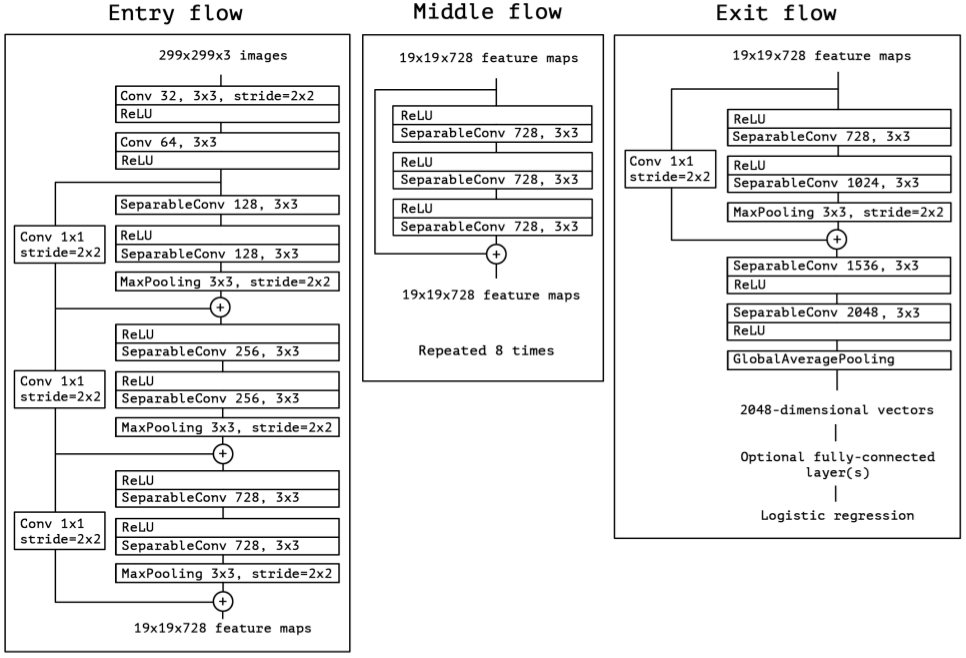
\includegraphics[width=\textwidth]{img/xception}
    \caption{Structure of \textit{Xception} architecture. Taken from \cite[fig. 5]{bib:xception}.}
    \label{fig:xception}
\end{figure}


\subsection{NASNet (2017)}
\label{sec:nasnet}
The difference between this architecture and the others mentioned is that \citeauthor{bib:nasnet} \cite{bib:nasnet} used a machine learning algorithm to design the network. It is a result of a \textit{AutoML}\footnote{\url{https://ai.googleblog.com/2017/05/using-machine-learning-to-explore.html}} project that automates the design of network architecture. Unlike manually designing the network by trial and error, \textit{AutoML} searches space of all possible models, e.g., using reinforcement learning and evolutionary algorithms. The downside of this approach is the computational cost and therefore limitation to small datasets.

\textit{NASNet} is a result of taking an architecture designed for small dataset (\textit{CIFAR-10}\footnote{\url{https://www.cs.toronto.edu/~kriz/cifar.html}}) by \textit{AutoML} and using it to create larger model for \textit{ImageNet} dataset. The model is composed of two types of learned cells, a \textit{Normal Cell} and \textit{Reduction Cell} (see \cref{fig:nasnet}). A general structure of the network is then created by alternating a \textit{Reduction Cell} and \textbf{N} \textit{Normal Cells}

\begin{figure}
    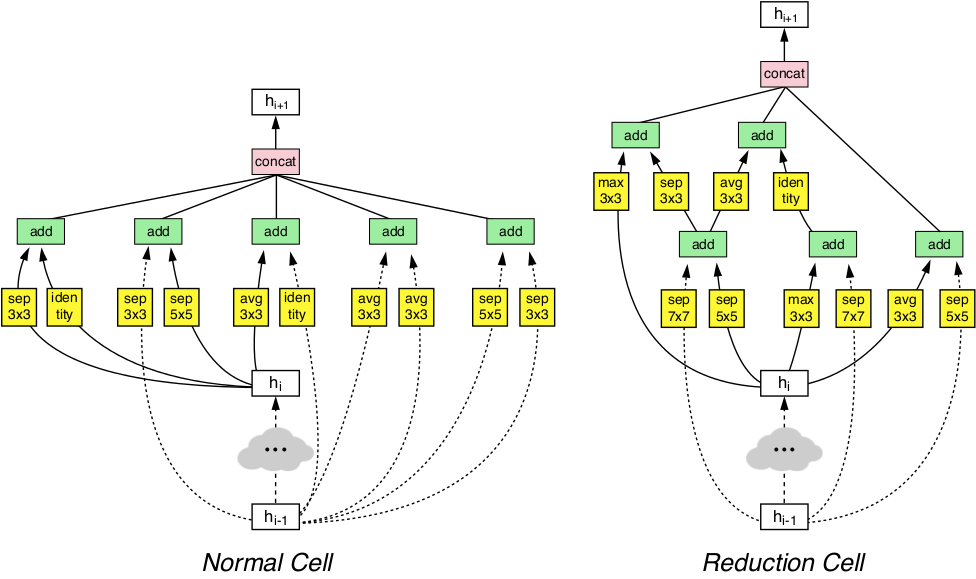
\includegraphics[width=\textwidth]{img/nasnet}
    \caption{Layers used in \textit{NASNet-A}, designed by \textit{AutoML}. Image from \url{ai.googleblog.com/2017/11/automl-for-large-scale-image}.}
    \label{fig:nasnet}
\end{figure}

\subsection{Comparing the classifiers}
At the beginning of this chapter, we mentioned that the classification networks are often compared based on performance on the \textit{ILSVRC} dataset. Newer models, like \textit{Xception}, \textit{NASNet}, and modifications of \textit{ResNet} reach excellent accuracy. However, there is a large discrepancy in their performance considering inference speed. In \cref{fig:cnnbenchmark} we provide an overview of fps-accuracy relationship taken from an independent benchmark by \citeauthor{bib:cnnbenchmark} \cite{bib:cnnbenchmark}. Although the experiment was performed with batch size 1, we expect a universal increase of fps with a bigger batch and only small changes to the relative performance of different models. We can observe a clear trade-off between speed and accuracy for the classification task.

\begin{figure}
    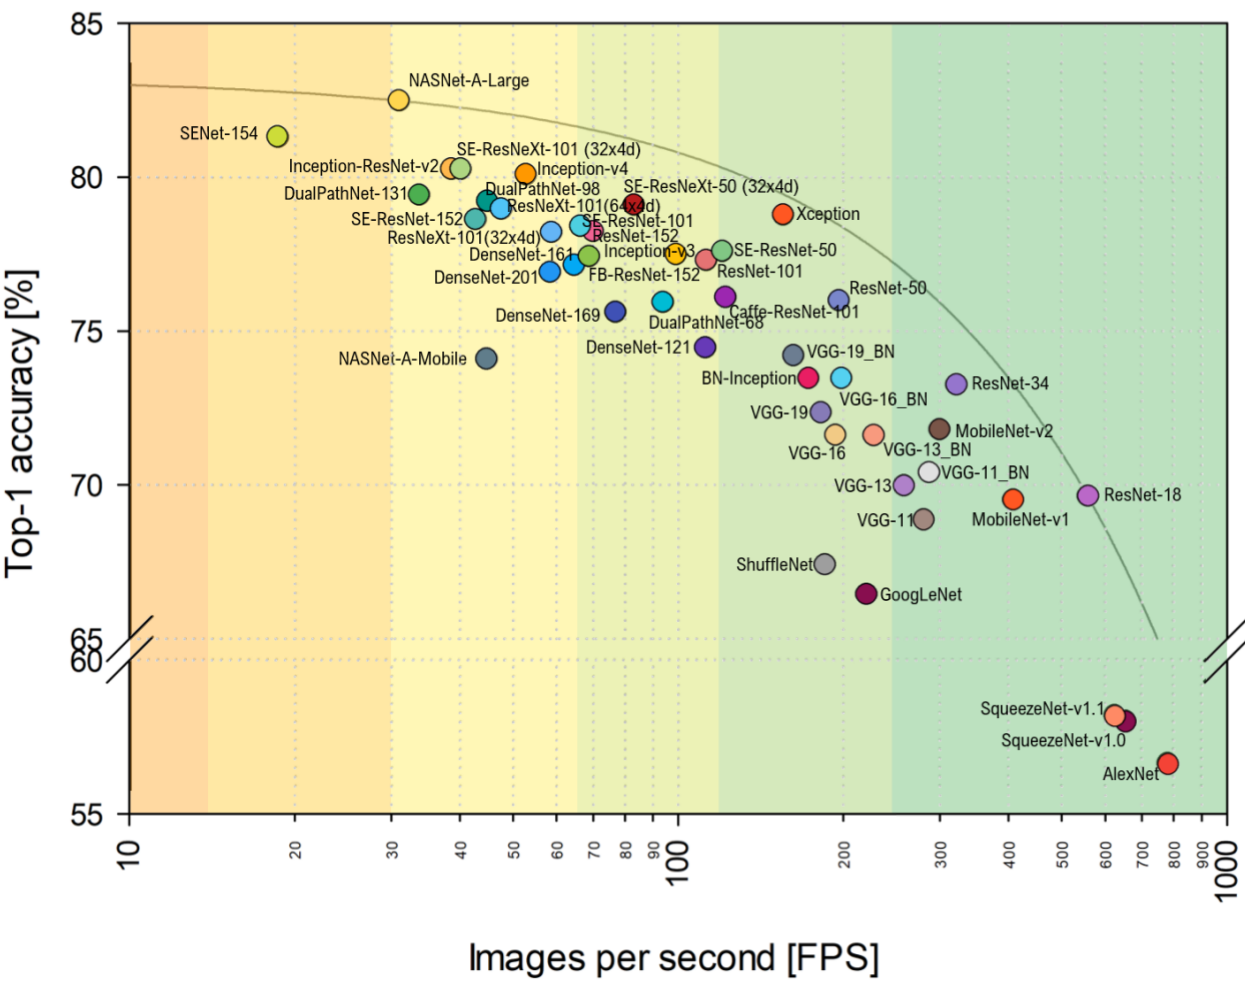
\includegraphics[width=\textwidth]{img/fps_comp}
    \caption{Benchmark of state-of-the-art classification deep neural networks on \textit{ILSVRC} dataset. Performed on NVIDIA
Titan X GPU with batch size 1. Taken from \cite[fig. 3]{bib:cnnbenchmark}}
    \label{fig:cnnbenchmark}
\end{figure}



\section{Detection networks}
\label{sec:detnets}
The goal of the detection network is to localize all objects of chosen categories. There is a simple logical step from classification task to detection. It is to classify selected regions in the image as one of the classes or as a background. Classification applied to every possible box in the image would undoubtedly produce great detection results, but at the extreme computational cost. This section describes a family of algorithms based on this simple idea, and try to implement it more efficiently.

We will see that this family of so-called \textit{region based} approaches can reach state-of-the-art results, with increasing efficiency with each generation. Considering precision, \textit{Faster R-CNN} is still used as one of the most reliable detectors. However, although it can process a few frames per second, we do not consider it to be a truly real-time detector and applicable for demanding tasks, such as video surveillance. We devote entire \cref{chap:rltm} to detection networks performing in real-time constraints.

\subsection{R-CNN (2014)}
Region-based Convolutional Network (\textit{R-CNN}) by \citeauthor{bib:rcnn} \cite{bib:rcnn} is the first member of the family of region-based detection models. Each iteration comes with improvements in speed and accuracy. The foundation idea is simple: select regions in the picture and classify each region. This approach leads to a combination of three modules: region proposal algorithm, feature extraction using CNNs on those regions and subsequent classification. 

A naive approach would use a sliding window and classify each cutout of the image. Considering windows for different sizes and aspect ratios of possible objects, this approach would be extremely slow. \textit{R-CNN} solves this problem by applying a region proposal algorithm that selects about 2000 most likely locations of objects. Regions are selected using the \textit{Selective search} \cite{bib:selectivesearch} algorithm and serve as a candidates for bbox predictions. In addition, bounding box regression can be trained to improve bbox prediction accuracy.

Each region is processed separately by a CNN into a feature map. The original architecture uses \textit{Alexnet}, but any classification network can be substituted. Finally, each feature map can be scored. \textit{R-CNN} uses class specific linear support-vector machines instead of a soft-max classification provided by classification CNNs. \Cref{fig:rcnn} illustrates the architecture.

\begin{figure}
    \centering
    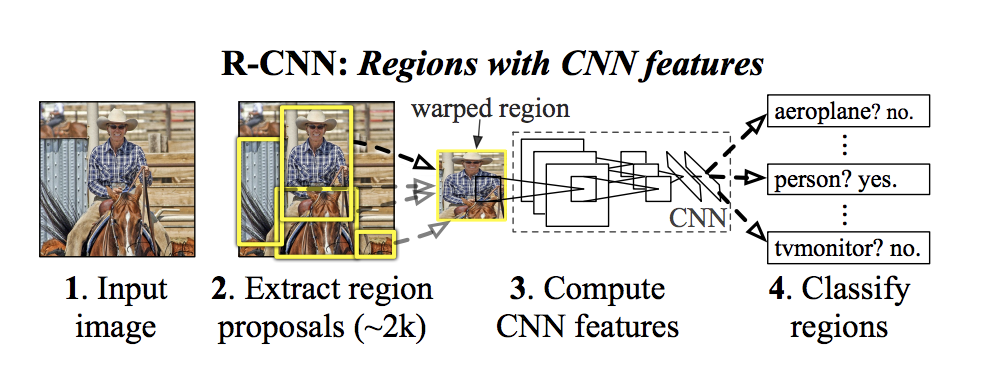
\includegraphics[width=\textwidth]{img/rcnn}
    \caption{R-CNN architecture. Taken from \cite[fig. 1]{bib:rcnn}.}
    \label{fig:rcnn}
\end{figure}

\subsection{Fast R-CNN (2015)}
Even though \textit{R-CNN} was a major step in the right direction, its performance is far from real-time detection. \citeauthor{bib:fastrcnn} \cite{bib:fastrcnn} introduces \textit{Fast R-CNN} with a series of innovations to its predecessor, aimed at improving speed and accuracy. Provided benchmark on the NVIDIA K40 GPU suggests improvements from 47 seconds per image using \textit{R-CNN} with \textit{VGG-16} feature extractor, to 320 milliseconds with \textit{Fast R-CNN} using the same feature extractor, not including a time for SS proposals. 

Similarly to \textit{R-CNN}, this architecture also utilizes region proposal algorithm and a CNN to produce a feature map. A significant drawback of \textit{R-CNN} was computing feature map for each region, despite overlaps. \textit{Fast R-CNN} processes whole input image into a feature map, and then, using a region of interest (RoI) pooling layers, extracts a feature vector for each region. All extracted feature vectors have the same size and are passed through a series of fully connected layers, leading to softmax classifier and bounding box regression layer. An illustration of this process can be seen on \cref{fig:fastrcnn}.

\begin{figure}
    \centering
    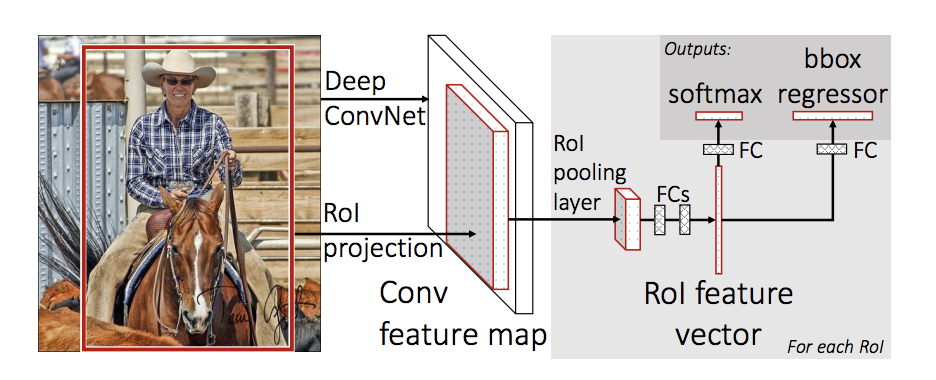
\includegraphics[width=\textwidth]{img/fastrcnn}
    \caption{Fast R-CNN architecture. Taken from \cite[fig. 1]{bib:fastrcnn}}
    \label{fig:fastrcnn}
\end{figure}

\subsection{Faster R-CNN (2015)}
 
 \textit{Faster R-CNN} by \citeauthor{bib:fasterrcnn} \cite{bib:fasterrcnn} expands on the \textit{Fast R-CNN} with the aspiration to achieve a real-time performance. \textit{Fast R-CNN} managed to build a fast feature extraction and subsequent classification usable in a real-time environment but is heavily slowed down by a region proposal SS algorithm. \textit{Faster R-CNN} expands on the idea of sharing resources and replaces selective search with \textit{region proposal network} (RPN). RPN is built on top of a feature map generated by the feature extractor. As suggested, the feature map is shared between RPN and object detection. This approach is able to achieve 5 fps, which can find limited use in a real-time environment. Whole architecture can be seen on \cref{fig:fasterrcnn}. 
 
 RPN is designed as a small, sliding-window network, with negligible cost compared to the feature extractor. It is composed of 3$\times$3 convolutional layer with 512 filters and two sibling 1$\times$1 convolutional layers for region regression and classification. Classification in RPNs determines whether proposed region contains an object or a background (\textit{cls} score). Region regression part of the network is tied to the concept of \textit{anchors}. The anchor is a predefined box centered at a location of sliding-window. Assuming \textit{k} anchors with different sizes and aspect ratios are used, regression produces 4k relative parameters and classifier 2k scores. Regression parameters are used to modify the position and size of their corresponding anchor. The number of regions is then reduced by eliminating proposals with high overlap using a non-maximum suppression (NMS) based on \textit{cls} score. After NMS, top-N ranked proposal regions are used for detection.
 
 To calculate loss and train RPN, a matching between ground-truth boxes and generated region proposals needs to be determined. A positive label is assigned to two kinds of regions: the one with the highest IoU overlap with ground-truth box; regions that have IoU higher than 0.7 with any ground-truth box. A negative label is assigned to a non-positive box if its IoU is lower than 0.3 for all ground-truth boxes. Rest of the boxes do not contribute to training. 
 
 The whole model is trained using a 4-step alternating training:
 
 \begin{enumerate}
     \item train RPN with feature extractor initialized by ImageNet pre-trained model
     \item train separate \textit{Fast R-CNN} using proposals generated by RPN from step 1
     \item train RPN with feature extractor initialized by weights learned by the detector in step 2, fine-tune only layers unique to RPN
     \item using the model from step 3, fine-tune layers unique to \textit{Fast R-CNN}
 \end{enumerate}

Thanks to the modular architecture, \textit{R-CNN} family networks can exploit any CNN as a feature extractor.  Therefore \textit{Faster R-CNN} can achieve state-of-the-art detection results exploiting the latest advances in classification networks and is often used as a benchmark of their performance.
     

 \begin{figure}
     \centering
     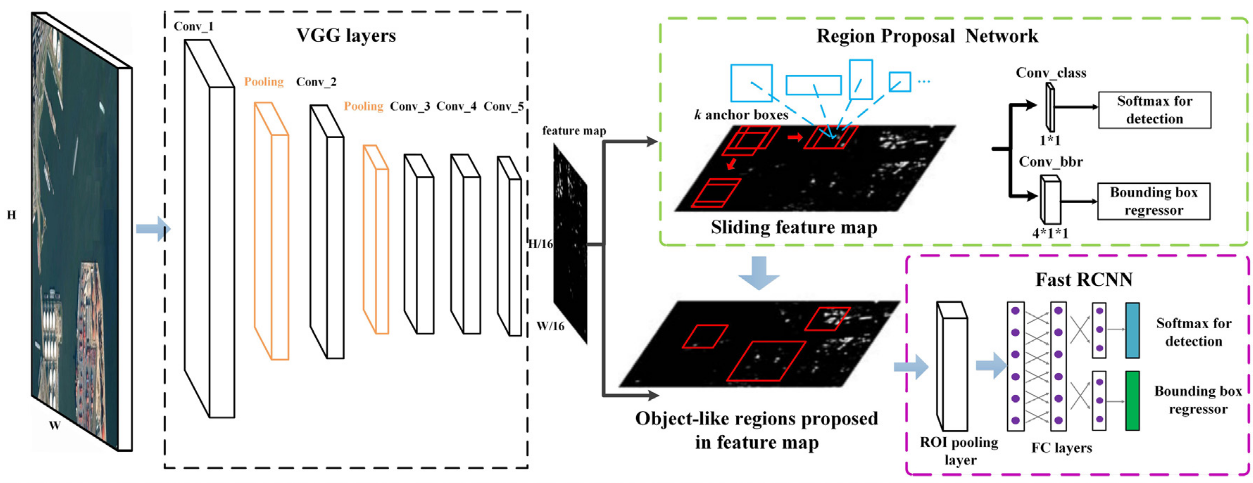
\includegraphics[width=\textwidth]{img/fasterrcnn}
     \caption{The architecture of Faster R-CNN. From \url{https://researchgate.net/figure/The-architecture-of-Faster-R-CNN\_fig2\_324903264}.}
     \label{fig:fasterrcnn}
 \end{figure}

 \subsection{Mask R-CNN (2017)}
Previous \textit{R-CNN} based architectures used bounding boxes to localize individual objects. \citeauthor{bib:maskrcnn} \cite{bib:maskrcnn} adds a localization based on semantic segmentation, where the goal is to classify each pixel into a category. \textit{Mask R-CNN} is built upon \textit{Faster R-CNN} and combines both bounding box localization and semantic segmentation by predicting segmentation masks for each RoI. The product of this approach is a bounding box and class for each object, together with a binary segmentation mask. Unlike the semantic segmentation on whole input, applying it on RoIs allows for instantiated segmentation where selected pixels corresponds to a given instance of a class.

Implementation and architecture are very similar to \textit{Faster R-CNN}, with two exceptions. One of them is already described, fully convolutional segmentation branch which works in parallel with classification and bounding box regression heads. The other difference is a replacement of RoI pooling layer with RoI alignment layer. The problem of RoI pooling for this purpose is quantization of floating-number RoI to discrete feature map grid and consequent imprecision. RoI align mitigates this problem by using bi-linear interpolation to compute exact values of features at four sampled location in each of RoIs locations and aggregating the results. High-level architecture and RoI alignment layer are visualized on \cref{fig:maskrcnn}.

 \begin{figure}
     \centering
     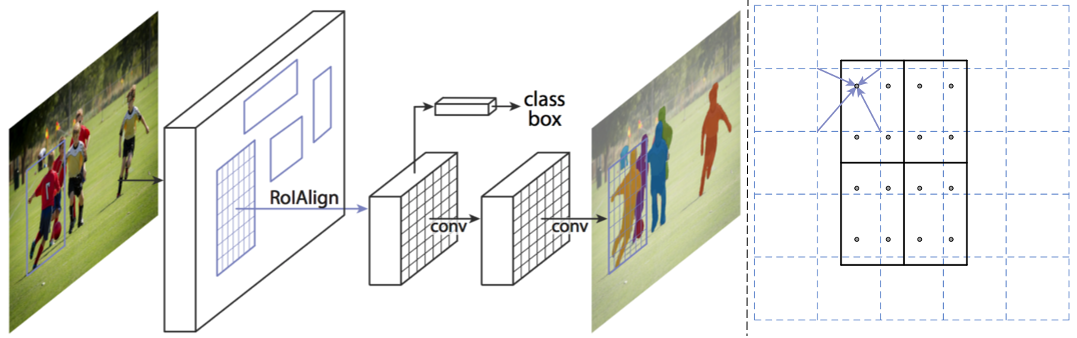
\includegraphics[width=\textwidth]{img/maskrcnn}
     \caption{Left: The architecture of Mask R-CNN. Right: RoI align, grid represents feature map, solid lines an RoI and the dost are the sampling points. From \cite[fig. 1, 3]{bib:maskrcnn}}
     \label{fig:maskrcnn}
 \end{figure}


